\documentclass[notheorems]{beamer}
\usepackage{latexsym}
\usepackage{amsmath,amssymb}
\usepackage{color,xcolor}
\usepackage{graphicx}
\usepackage{algorithm}
\usepackage{amsthm}
\usepackage[UTF8]{ctex}
\usepackage{subfigure}

%\usetheme{Madrid}
%\usetheme{AnnArbor}
%\usetheme{Antibes}
%\usetheme{Bergen}
%\usetheme{Berkeley}
%\usetheme{Berlin}
%\usetheme{Boadilla}
\usetheme{boxes}
%\usetheme{CambridgeUS}
%\usetheme{Copenhagen}
%\usetheme{Darmstadt}
%\usetheme{default}
%\usetheme{Frankfurt}
%\usetheme{Goettingen}
%\usetheme{Hannover}
%\usetheme{Ilmenau}
%\usetheme{JuanLesPins}
%\usetheme{Luebeck}
%\usetheme{Madrid}
%\usetheme{Malmoe}
%\usetheme{Marburg}
%\usetheme{Montpellier}
%\usetheme{PaloAlto}
%\usetheme{Pittsburgh}
%\usetheme{Rochester}
%\usetheme{Singapore}
%\usetheme{Szeged}
%\usetheme{Warsaw}

\usefonttheme[onlymath]{serif}
\usecolortheme{whale}
%\newtheorem{proposition}{Proposition}
\newtheorem{proposition}{命题}
\newtheorem{theorem}{定理}
\newtheorem{definition}{定义}
\newtheorem{example}{例}

\renewcommand\figurename{图}
\renewcommand\tablename{表}

\setbeamertemplate{theorems}[numbered]
\begin{document}

\title[CHIVOX]{Doc2vec 模型结构和训练}
\author[mf34]{方敏}
\institute[Department of Research] {驰声研发}
\date[Oct, 2016]{2016 年 10月}

\frame{\titlepage}

\begin{frame}
\frametitle{overview}
\begin{itemize}
\item 背景知识:word2vec模型
\item Doc2vec模型结构介绍
\item 模型训练与doc向量获取 %包括语料训练和文档向量的生成
\item Optimizing Computational Efficiency
\item 其它模型
\end{itemize}
\end{frame}

\begin{frame}
\frametitle{背景知识:word2vec模型}
 \begin{minipage}[t]{0.4\linewidth}
 \centering
     \begin{figure}
      \scalebox{0.30}
      {
        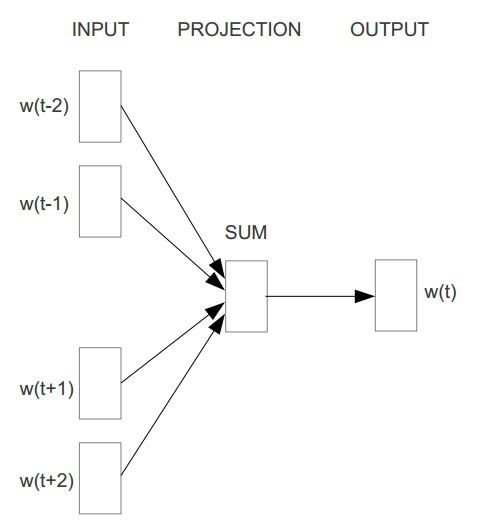
\includegraphics{./figure/CBOW.png}
      }
      \caption{CBOW(Continuous Bag-of-Words Model)}
    \end{figure}
 \end{minipage}%
\begin{minipage}[t]{0.5\linewidth}
\centering
\begin{itemize}
\item 预测$p(w_{t}|w_{t-k},...,w_{t+k})$
\item 目标函数如下
\begin{equation}
\begin{aligned}
& \dfrac{1}{T}\sum_{t=k}^{T-k}logp(w_{t}|w_{t-k},...,w_{t+k})\\
& p(w_{t}|w_{t-k},...,w_{t+k})=\dfrac{e^{y_{w_{t}}}}{\sum_{i}e^{y_{i}}}\\
& y_{w_{t}}=b + Uh(w_{t-k},...w_{t+k})
\end{aligned}
\end{equation}
\begin{footnotesize}
$h$表示INPUT到PROJECTION的转化关系,如求和
\end{footnotesize}
\end{itemize}
\end{minipage}     
\end{frame}

\begin{frame}
\frametitle{Doc2vec模型结构介绍}
     
 \begin{minipage}[t]{0.4\linewidth}
 \centering
     \begin{figure}
      \scalebox{0.25}
      {
        \includegraphics{./figure/skip-gram.png}
      }
      \caption{Doc2vec PV-DM}
    \end{figure}
 \end{minipage}%
\begin{minipage}[t]{0.6\linewidth}
\centering
\begin{itemize}
\item 预测
$p(w_{t,j}|w_{t-k,j},...,w_{t+k,j},d^{j})$\\
\begin{footnotesize}
$w_{t,j}$表示第$j$篇doc的第$t$个词,$d^{j}$表示第$j$篇doc,$k$为$1/2$窗长\\
\end{footnotesize}
\item 分类器
\begin{equation}
\begin{aligned}
& p(w_{t,j}|w_{t-k,j},...,w_{t+k,j})=\dfrac{e^{y_{w_{t,j}}}}{\sum_{i}e^{y_{i}}}\\
& y_{w_{t,j}}=b + Uh(w_{t-k,j},...w_{t+k,j},d_{j})
\end{aligned}
\end{equation}
\end{itemize}

\end{minipage}     
\end{frame}


\begin{frame}
\frametitle{Doc2vec模型结构介绍}
\begin{flushleft}
目标函数:
\begin{equation}
\frac{1}{J}\sum_{j=1}^{J}\frac{1}{N_{j}-2k}\sum_{t=k}^{N_{j}-k}logp(w_{t,j}|w_{t-k,j},...,w_{t+k,j},d_{j})
\end{equation}
其中,$N_{j}$表示第$j$篇doc的字符长度,$J$表示语料中包含的doc数目
\end{flushleft}
\end{frame}



\begin{frame}
\frametitle{模型训练与doc向量获取}
若不考虑使用输出反馈:
\begin{equation}
h_{t}=f(W_{xh}x_t+W_{hh}h_{t-1})
\end{equation}
\begin{equation}
y_{t}=g(W_{hy}h_{t})
\end{equation}

\end{frame}

\begin{frame}
\frametitle{Optimizing Computational Efficiency}
\begin{itemize}
\item Negative Sampling
\item Hierarchical Softmax
\begin{equation}
\begin{aligned}
& \dfrac{1}{T}\sum_{t=k}^{T-k}logp(w_{t}|w_{t-k},...,w_{t+k})\\
& p(w_{t}|w_{t-k},...,w_{t+k})=\dfrac{e^{y_{w_{t}}}}{\sum_{i}e^{y_{i}}}\\
& y_{w_{t}}=b + Uh(w_{t-k},...w_{t+k})
\end{aligned}
\end{equation}
\end{itemize}

\end{frame}

\begin{frame}
\frametitle{其它模型}
 \begin{minipage}[t]{0.4\linewidth}
 \centering
     \begin{figure}
      \scalebox{0.30}
      {
        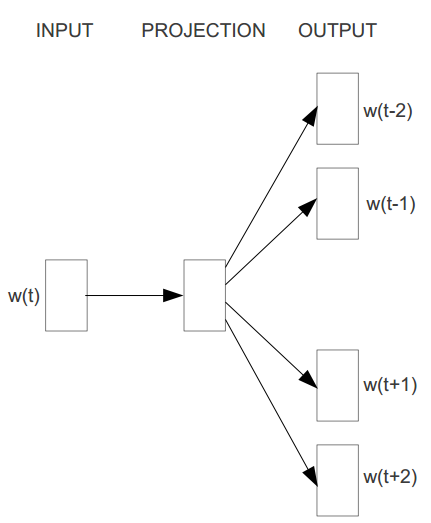
\includegraphics{./figure/Skip-Gram.png}
      }
      \caption{CBOW(Continuous Bag-of-Words Model)}
    \end{figure}
 \end{minipage}%
\begin{minipage}[t]{0.5\linewidth}
\centering
\begin{itemize}
\item 预测$p(w_{t}|w_{t-k},...,w_{t+k})$
\item 目标函数如下
\begin{equation}
\begin{aligned}
& \dfrac{1}{T}\sum_{t=k}^{T-k}\sum_{-k<=l<=k,l!=0}logp(w_{t+l}|w_{t})\\
& p(w|w_{t})=\dfrac{e^{y_{w}}}{\sum_{i}e^{y_{i}}}\\
& y_{w}=b + Uh(w_{t})
\end{aligned}
\end{equation}
\end{itemize}

\end{minipage}     
\end{frame}

\begin{frame}
\frametitle{其它模型}
\begin{figure}
\begin{minipage}[t]{0.5\linewidth}
\centering	
\includegraphics[width=2in]{./figure/skip-gram.png}
\caption{Doc2vec PV-DM}
\label{fig:side:a}	
\end{minipage}%
\begin{minipage}[t]{0.5\linewidth}
\centering
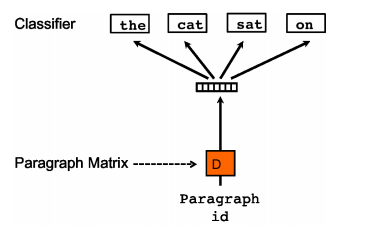
\includegraphics[width=2.2in]{./figure/Distributed_bag_of_word.png}
\caption{Doc2vec PV-DBOW}		
\label{fig:side:b}	
\end{minipage}
\end{figure}
\end{frame}

\end{document}
